\documentclass{standalone}
\usepackage{tikz}
\usetikzlibrary{patterns, positioning}
\usepackage[sfdefault]{ClearSans} %% option 'sfdefault' activates Clear Sans as the default text font
\usepackage[T1]{fontenc}

\begin{document}
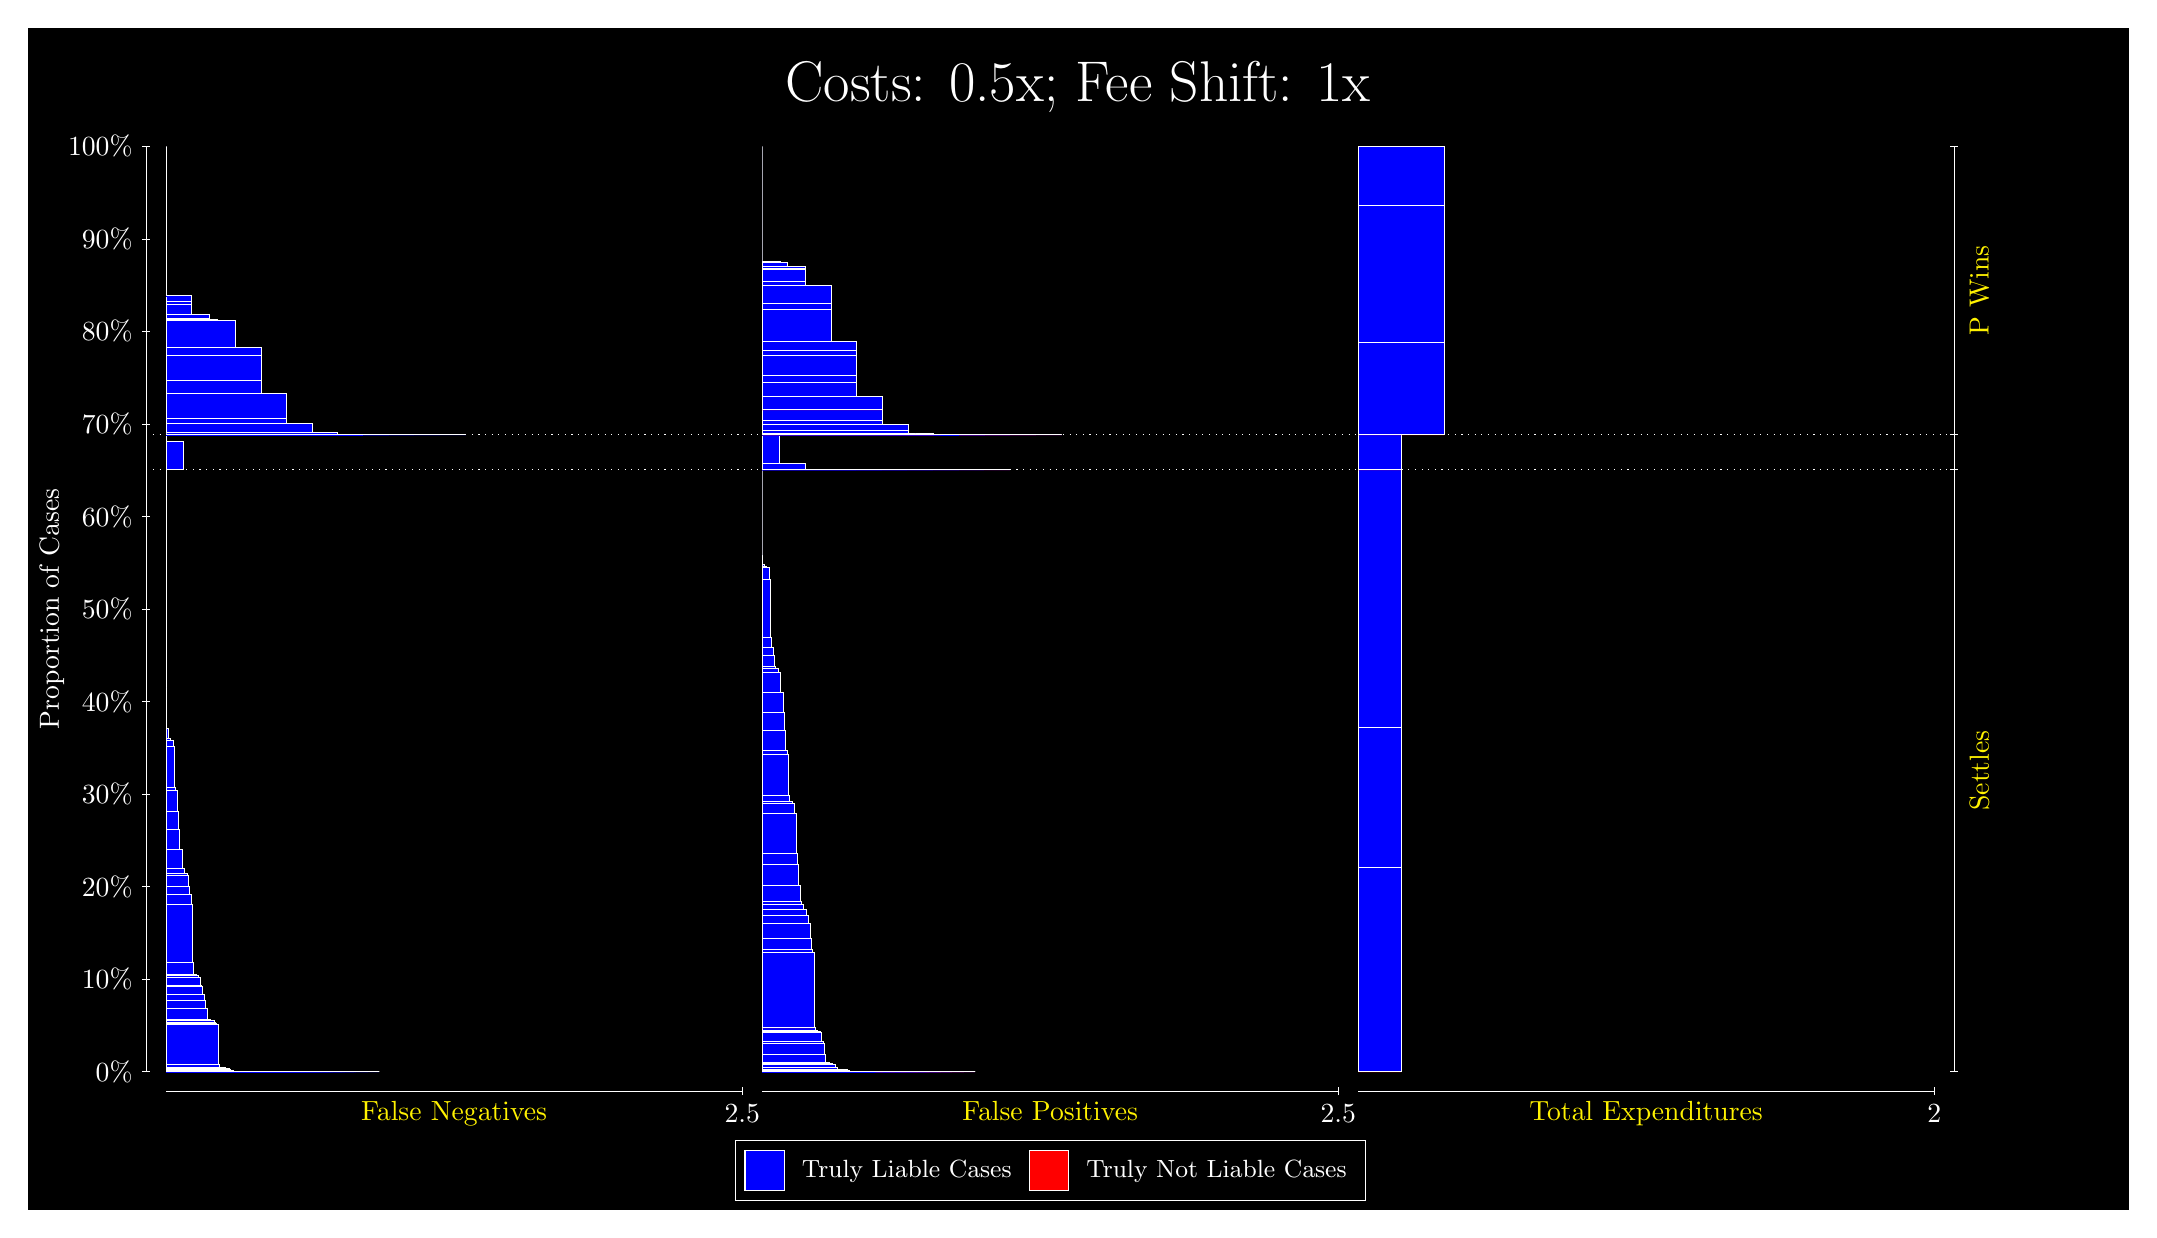
\begin{tikzpicture}
\draw[fill=black] (0,0) rectangle (26.667,15);
\draw[text=white] (0,13.5) rectangle (26.667,15) node[midway] {\huge Costs: 0.5x; Fee Shift: 1x};
\draw[white, very thin] (1.5,1.75) -- (1.5,13.5);
\node[rotate=90, text=white, anchor=center] at (0.3, 7.625) {Proportion of Cases};
\draw[white, very thin] (1.45,1.75) -- (1.55,1.75);
\node[text=white, anchor=east] at (1.45, 1.75) {0\%};
\draw[white, very thin] (1.45,2.925) -- (1.55,2.925);
\node[text=white, anchor=east] at (1.45, 2.925) {10\%};
\draw[white, very thin] (1.45,4.1) -- (1.55,4.1);
\node[text=white, anchor=east] at (1.45, 4.1) {20\%};
\draw[white, very thin] (1.45,5.275) -- (1.55,5.275);
\node[text=white, anchor=east] at (1.45, 5.275) {30\%};
\draw[white, very thin] (1.45,6.45) -- (1.55,6.45);
\node[text=white, anchor=east] at (1.45, 6.45) {40\%};
\draw[white, very thin] (1.45,7.625) -- (1.55,7.625);
\node[text=white, anchor=east] at (1.45, 7.625) {50\%};
\draw[white, very thin] (1.45,8.8) -- (1.55,8.8);
\node[text=white, anchor=east] at (1.45, 8.8) {60\%};
\draw[white, very thin] (1.45,9.975) -- (1.55,9.975);
\node[text=white, anchor=east] at (1.45, 9.975) {70\%};
\draw[white, very thin] (1.45,11.15) -- (1.55,11.15);
\node[text=white, anchor=east] at (1.45, 11.15) {80\%};
\draw[white, very thin] (1.45,12.325) -- (1.55,12.325);
\node[text=white, anchor=east] at (1.45, 12.325) {90\%};
\draw[white, very thin] (1.45,13.5) -- (1.55,13.5);
\node[text=white, anchor=east] at (1.45, 13.5) {100\%};

\draw[white, very thin] (24.457,1.75) -- (24.457,13.5);
\draw[white, very thin] (24.407,1.75) -- (24.507,1.75);
\node[anchor=west] at (24.407, 1.75) {};
\draw[white, very thin] (24.407,9.3939) -- (24.507,9.3939);
\node[anchor=west] at (24.407, 9.3939) {};
\draw[white, very thin] (24.407,9.8375) -- (24.507,9.8375);
\node[anchor=west] at (24.407, 9.8375) {};
\draw[white, very thin] (24.407,13.5) -- (24.507,13.5);
\node[anchor=west] at (24.407, 13.5) {};

\draw[white, very thin, fill=blue] (1.75,1.75) rectangle (4.458,1.75);
\draw[white, very thin, fill=blue] (1.75,1.75) rectangle (4.3116,1.75);
\draw[white, very thin, fill=blue] (1.75,1.75) rectangle (4.1652,1.75);
\draw[white, very thin, fill=blue] (1.75,1.75) rectangle (4.1327,1.75);
\draw[white, very thin, fill=blue] (1.75,1.75) rectangle (4.0188,1.75);
\draw[white, very thin, fill=blue] (1.75,1.75) rectangle (3.9863,1.75);
\draw[white, very thin, fill=blue] (1.75,1.75) rectangle (3.8725,1.75);
\draw[white, very thin, fill=blue] (1.75,1.75) rectangle (3.8399,1.75);
\draw[white, very thin, fill=blue] (1.75,1.75) rectangle (3.8074,1.75);
\draw[white, very thin, fill=blue] (1.75,1.75) rectangle (3.7261,1.75);
\draw[white, very thin, fill=blue] (1.75,1.75) rectangle (3.6936,1.75);
\draw[white, very thin, fill=blue] (1.75,1.75) rectangle (3.661,1.75);
\draw[white, very thin, fill=blue] (1.75,1.75) rectangle (3.5797,1.75);
\draw[white, very thin, fill=blue] (1.75,1.75) rectangle (3.5472,1.75);
\draw[white, very thin, fill=blue] (1.75,1.75) rectangle (3.5147,1.75);
\draw[white, very thin, fill=blue] (1.75,1.75) rectangle (3.4821,1.75);
\draw[white, very thin, fill=blue] (1.75,1.75) rectangle (3.4333,1.75);
\draw[white, very thin, fill=blue] (1.75,1.75) rectangle (3.4008,1.75);
\draw[white, very thin, fill=blue] (1.75,1.75) rectangle (3.3683,1.75);
\draw[white, very thin, fill=blue] (1.75,1.75) rectangle (3.3358,1.75);
\draw[white, very thin, fill=blue] (1.75,1.75) rectangle (3.287,1.75);
\draw[white, very thin, fill=blue] (1.75,1.75) rectangle (3.2544,1.75);
\draw[white, very thin, fill=blue] (1.75,1.75) rectangle (3.2219,1.75);
\draw[white, very thin, fill=blue] (1.75,1.75) rectangle (3.1894,1.75);
\draw[white, very thin, fill=blue] (1.75,1.75) rectangle (3.1568,1.75);
\draw[white, very thin, fill=blue] (1.75,1.75) rectangle (3.1406,1.75);
\draw[white, very thin, fill=blue] (1.75,1.75) rectangle (3.1081,1.75);
\draw[white, very thin, fill=blue] (1.75,1.75) rectangle (3.0755,1.75);
\draw[white, very thin, fill=blue] (1.75,1.75) rectangle (3.043,1.75);
\draw[white, very thin, fill=blue] (1.75,1.75) rectangle (3.0105,1.75);
\draw[white, very thin, fill=blue] (1.75,1.75) rectangle (2.9942,1.75);
\draw[white, very thin, fill=blue] (1.75,1.75) rectangle (2.9617,1.75);
\draw[white, very thin, fill=blue] (1.75,1.75) rectangle (2.9292,1.7504);
\draw[white, very thin, fill=blue] (1.75,1.7504) rectangle (2.8966,1.7505);
\draw[white, very thin, fill=blue] (1.75,1.7505) rectangle (2.8641,1.7505);
\draw[white, very thin, fill=blue] (1.75,1.7505) rectangle (2.8478,1.7505);
\draw[white, very thin, fill=blue] (1.75,1.7505) rectangle (2.8316,1.7506);
\draw[white, very thin, fill=blue] (1.75,1.7506) rectangle (2.8153,1.7506);
\draw[white, very thin, fill=blue] (1.75,1.7506) rectangle (2.7828,1.7506);
\draw[white, very thin, fill=blue] (1.75,1.7506) rectangle (2.7502,1.7522);
\draw[white, very thin, fill=blue] (1.75,1.7522) rectangle (2.7177,1.7527);
\draw[white, very thin, fill=blue] (1.75,1.7527) rectangle (2.7015,1.753);
\draw[white, very thin, fill=blue] (1.75,1.753) rectangle (2.6852,1.7534);
\draw[white, very thin, fill=blue] (1.75,1.7534) rectangle (2.6689,1.7537);
\draw[white, very thin, fill=blue] (1.75,1.7537) rectangle (2.6364,1.7539);
\draw[white, very thin, fill=blue] (1.75,1.7539) rectangle (2.6039,1.7698);
\draw[white, very thin, fill=blue] (1.75,1.7698) rectangle (2.5713,1.7776);
\draw[white, very thin, fill=blue] (1.75,1.7776) rectangle (2.5551,1.788);
\draw[white, very thin, fill=blue] (1.75,1.788) rectangle (2.5388,1.794);
\draw[white, very thin, fill=blue] (1.75,1.794) rectangle (2.5225,1.7942);
\draw[white, very thin, fill=blue] (1.75,1.7942) rectangle (2.5063,1.7994);
\draw[white, very thin, fill=blue] (1.75,1.7994) rectangle (2.49,1.8013);
\draw[white, very thin, fill=blue] (1.75,1.8013) rectangle (2.4575,1.802);
\draw[white, very thin, fill=blue] (1.75,1.802) rectangle (2.425,1.8376);
\draw[white, very thin, fill=blue] (1.75,1.8376) rectangle (2.4087,2.3468);
\draw[white, very thin, fill=blue] (1.75,2.3468) rectangle (2.3924,2.3679);
\draw[white, very thin, fill=blue] (1.75,2.3679) rectangle (2.3762,2.3758);
\draw[white, very thin, fill=blue] (1.75,2.3758) rectangle (2.3599,2.3948);
\draw[white, very thin, fill=blue] (1.75,2.3948) rectangle (2.3436,2.4002);
\draw[white, very thin, fill=blue] (1.75,2.4002) rectangle (2.3111,2.4086);
\draw[white, very thin, fill=blue] (1.75,2.4086) rectangle (2.2786,2.5514);
\draw[white, very thin, fill=blue] (1.75,2.5514) rectangle (2.2461,2.6589);
\draw[white, very thin, fill=blue] (1.75,2.6589) rectangle (2.2298,2.7341);
\draw[white, very thin, fill=blue] (1.75,2.7341) rectangle (2.2135,2.8328);
\draw[white, very thin, fill=blue] (1.75,2.8328) rectangle (2.1973,2.8394);
\draw[white, very thin, fill=blue] (1.75,2.8394) rectangle (2.181,2.9481);
\draw[white, very thin, fill=blue] (1.75,2.9481) rectangle (2.1647,2.9776);
\draw[white, very thin, fill=blue] (1.75,2.9776) rectangle (2.1322,2.9882);
\draw[white, very thin, fill=blue] (1.75,2.9882) rectangle (2.0997,3.1438);
\draw[white, very thin, fill=blue] (1.75,3.1438) rectangle (2.0834,3.874);
\draw[white, very thin, fill=blue] (1.75,3.874) rectangle (2.0672,4.0049);
\draw[white, very thin, fill=blue] (1.75,4.0049) rectangle (2.0509,4.104);
\draw[white, very thin, fill=blue] (1.75,4.104) rectangle (2.0346,4.2417);
\draw[white, very thin, fill=blue] (1.75,4.2417) rectangle (2.0184,4.2721);
\draw[white, very thin, fill=blue] (1.75,4.2721) rectangle (1.9858,4.3253);
\draw[white, very thin, fill=blue] (1.75,4.3253) rectangle (1.9533,4.5769);
\draw[white, very thin, fill=blue] (1.75,4.5769) rectangle (1.9208,4.8296);
\draw[white, very thin, fill=blue] (1.75,4.8296) rectangle (1.9045,5.0574);
\draw[white, very thin, fill=blue] (1.75,5.0574) rectangle (1.8882,5.3188);
\draw[white, very thin, fill=blue] (1.75,5.3188) rectangle (1.872,5.3599);
\draw[white, very thin, fill=blue] (1.75,5.3599) rectangle (1.8557,5.8864);
\draw[white, very thin, fill=blue] (1.75,5.8864) rectangle (1.8395,5.9598);
\draw[white, very thin, fill=blue] (1.75,5.9598) rectangle (1.8069,5.9866);
\draw[white, very thin, fill=blue] (1.75,5.9866) rectangle (1.7744,6.1153);
\draw[white, very thin, fill=blue] (1.75,6.1153) rectangle (1.7581,6.6246);
\draw[white, very thin, fill=red] (1.75,6.6246) rectangle (1.75,6.6246);
\draw[white, very thin, fill=blue] (1.75,6.6246) rectangle (1.75,9.3939);
\draw[white, very thin, fill=blue] (1.75,9.3939) rectangle (1.9696,9.7543);
\draw[white, very thin, fill=red] (1.75,9.7543) rectangle (1.75,9.7543);
\draw[white, very thin, fill=blue] (1.75,9.7543) rectangle (1.75,9.8375);
\draw[white, very thin, fill=blue] (1.75,9.8375) rectangle (5.5558,9.8375);
\draw[white, very thin, fill=blue] (1.75,9.8375) rectangle (5.2305,9.8375);
\draw[white, very thin, fill=blue] (1.75,9.8375) rectangle (4.9052,9.8375);
\draw[white, very thin, fill=blue] (1.75,9.8375) rectangle (4.58,9.8376);
\draw[white, very thin, fill=blue] (1.75,9.8376) rectangle (4.58,9.8377);
\draw[white, very thin, fill=blue] (1.75,9.8377) rectangle (4.2547,9.8394);
\draw[white, very thin, fill=blue] (1.75,9.8394) rectangle (4.2547,9.8404);
\draw[white, very thin, fill=blue] (1.75,9.8404) rectangle (4.027,9.8404);
\draw[white, very thin, fill=blue] (1.75,9.8404) rectangle (3.9294,9.8631);
\draw[white, very thin, fill=blue] (1.75,9.8631) rectangle (3.7017,9.8631);
\draw[white, very thin, fill=blue] (1.75,9.8631) rectangle (3.7017,9.8631);
\draw[white, very thin, fill=blue] (1.75,9.8631) rectangle (3.6041,9.9813);
\draw[white, very thin, fill=blue] (1.75,9.9813) rectangle (3.3764,9.9813);
\draw[white, very thin, fill=blue] (1.75,9.9813) rectangle (3.2788,10.045);
\draw[white, very thin, fill=blue] (1.75,10.045) rectangle (3.2788,10.363);
\draw[white, very thin, fill=blue] (1.75,10.363) rectangle (3.0511,10.363);
\draw[white, very thin, fill=blue] (1.75,10.363) rectangle (3.0511,10.363);
\draw[white, very thin, fill=blue] (1.75,10.363) rectangle (2.9535,10.523);
\draw[white, very thin, fill=blue] (1.75,10.523) rectangle (2.9535,10.849);
\draw[white, very thin, fill=blue] (1.75,10.849) rectangle (2.9535,10.946);
\draw[white, very thin, fill=blue] (1.75,10.946) rectangle (2.7258,10.946);
\draw[white, very thin, fill=blue] (1.75,10.946) rectangle (2.7258,10.946);
\draw[white, very thin, fill=blue] (1.75,10.946) rectangle (2.7258,10.947);
\draw[white, very thin, fill=blue] (1.75,10.947) rectangle (2.6283,11.296);
\draw[white, very thin, fill=blue] (1.75,11.296) rectangle (2.4006,11.297);
\draw[white, very thin, fill=blue] (1.75,11.297) rectangle (2.4006,11.308);
\draw[white, very thin, fill=blue] (1.75,11.308) rectangle (2.303,11.312);
\draw[white, very thin, fill=blue] (1.75,11.312) rectangle (2.303,11.362);
\draw[white, very thin, fill=blue] (1.75,11.362) rectangle (2.303,11.366);
\draw[white, very thin, fill=blue] (1.75,11.366) rectangle (2.0753,11.498);
\draw[white, very thin, fill=blue] (1.75,11.498) rectangle (2.0753,11.529);
\draw[white, very thin, fill=blue] (1.75,11.529) rectangle (2.0753,11.602);
\draw[white, very thin, fill=blue] (1.75,11.602) rectangle (1.9777,11.603);
\draw[white, very thin, fill=blue] (1.75,11.603) rectangle (1.9777,11.603);
\draw[white, very thin, fill=red] (1.75,11.603) rectangle (1.75,11.603);
\draw[white, very thin, fill=blue] (1.75,11.603) rectangle (1.75,13.5);
\draw[white, very thin, fill=red] (9.3189,1.75) rectangle (12.027,1.75);
\draw[white, very thin, fill=blue] (9.3189,1.75) rectangle (12.027,1.75);
\draw[white, very thin, fill=red] (9.3189,1.75) rectangle (11.88,1.75);
\draw[white, very thin, fill=blue] (9.3189,1.75) rectangle (11.88,1.75);
\draw[white, very thin, fill=red] (9.3189,1.75) rectangle (11.734,1.75);
\draw[white, very thin, fill=blue] (9.3189,1.75) rectangle (11.734,1.75);
\draw[white, very thin, fill=blue] (9.3189,1.75) rectangle (11.702,1.75);
\draw[white, very thin, fill=red] (9.3189,1.75) rectangle (11.588,1.75);
\draw[white, very thin, fill=blue] (9.3189,1.75) rectangle (11.588,1.75);
\draw[white, very thin, fill=blue] (9.3189,1.75) rectangle (11.555,1.75);
\draw[white, very thin, fill=red] (9.3189,1.75) rectangle (11.441,1.75);
\draw[white, very thin, fill=blue] (9.3189,1.75) rectangle (11.441,1.75);
\draw[white, very thin, fill=blue] (9.3189,1.75) rectangle (11.409,1.75);
\draw[white, very thin, fill=blue] (9.3189,1.75) rectangle (11.376,1.75);
\draw[white, very thin, fill=red] (9.3189,1.75) rectangle (11.295,1.75);
\draw[white, very thin, fill=blue] (9.3189,1.75) rectangle (11.295,1.75);
\draw[white, very thin, fill=blue] (9.3189,1.75) rectangle (11.262,1.75);
\draw[white, very thin, fill=blue] (9.3189,1.75) rectangle (11.23,1.75);
\draw[white, very thin, fill=red] (9.3189,1.75) rectangle (11.149,1.75);
\draw[white, very thin, fill=blue] (9.3189,1.75) rectangle (11.149,1.75);
\draw[white, very thin, fill=blue] (9.3189,1.75) rectangle (11.116,1.75);
\draw[white, very thin, fill=blue] (9.3189,1.75) rectangle (11.084,1.75);
\draw[white, very thin, fill=blue] (9.3189,1.75) rectangle (11.051,1.75);
\draw[white, very thin, fill=red] (9.3189,1.75) rectangle (11.002,1.75);
\draw[white, very thin, fill=blue] (9.3189,1.75) rectangle (11.002,1.75);
\draw[white, very thin, fill=blue] (9.3189,1.75) rectangle (10.97,1.75);
\draw[white, very thin, fill=blue] (9.3189,1.75) rectangle (10.937,1.75);
\draw[white, very thin, fill=blue] (9.3189,1.75) rectangle (10.905,1.75);
\draw[white, very thin, fill=red] (9.3189,1.75) rectangle (10.856,1.75);
\draw[white, very thin, fill=blue] (9.3189,1.75) rectangle (10.856,1.75);
\draw[white, very thin, fill=blue] (9.3189,1.75) rectangle (10.823,1.75);
\draw[white, very thin, fill=blue] (9.3189,1.75) rectangle (10.791,1.75);
\draw[white, very thin, fill=blue] (9.3189,1.75) rectangle (10.758,1.7503);
\draw[white, very thin, fill=blue] (9.3189,1.7503) rectangle (10.726,1.7504);
\draw[white, very thin, fill=red] (9.3189,1.7504) rectangle (10.709,1.7504);
\draw[white, very thin, fill=blue] (9.3189,1.7504) rectangle (10.709,1.7504);
\draw[white, very thin, fill=blue] (9.3189,1.7504) rectangle (10.677,1.7504);
\draw[white, very thin, fill=blue] (9.3189,1.7504) rectangle (10.644,1.7504);
\draw[white, very thin, fill=blue] (9.3189,1.7504) rectangle (10.612,1.7506);
\draw[white, very thin, fill=blue] (9.3189,1.7506) rectangle (10.579,1.7521);
\draw[white, very thin, fill=red] (9.3189,1.7521) rectangle (10.563,1.7521);
\draw[white, very thin, fill=blue] (9.3189,1.7521) rectangle (10.563,1.7522);
\draw[white, very thin, fill=blue] (9.3189,1.7522) rectangle (10.531,1.7523);
\draw[white, very thin, fill=blue] (9.3189,1.7523) rectangle (10.498,1.7525);
\draw[white, very thin, fill=blue] (9.3189,1.7525) rectangle (10.465,1.7531);
\draw[white, very thin, fill=blue] (9.3189,1.7531) rectangle (10.433,1.7688);
\draw[white, very thin, fill=red] (9.3189,1.7688) rectangle (10.417,1.7688);
\draw[white, very thin, fill=blue] (9.3189,1.7688) rectangle (10.417,1.77);
\draw[white, very thin, fill=blue] (9.3189,1.77) rectangle (10.4,1.7753);
\draw[white, very thin, fill=blue] (9.3189,1.7753) rectangle (10.384,1.7758);
\draw[white, very thin, fill=blue] (9.3189,1.7758) rectangle (10.352,1.7765);
\draw[white, very thin, fill=blue] (9.3189,1.7765) rectangle (10.319,1.7783);
\draw[white, very thin, fill=blue] (9.3189,1.7783) rectangle (10.287,1.7848);
\draw[white, very thin, fill=red] (9.3189,1.7848) rectangle (10.27,1.7848);
\draw[white, very thin, fill=blue] (9.3189,1.7848) rectangle (10.27,1.803);
\draw[white, very thin, fill=blue] (9.3189,1.803) rectangle (10.254,1.8407);
\draw[white, very thin, fill=blue] (9.3189,1.8407) rectangle (10.238,1.8476);
\draw[white, very thin, fill=blue] (9.3189,1.8476) rectangle (10.205,1.8533);
\draw[white, very thin, fill=blue] (9.3189,1.8533) rectangle (10.173,1.8616);
\draw[white, very thin, fill=blue] (9.3189,1.8616) rectangle (10.14,1.8729);
\draw[white, very thin, fill=red] (9.3189,1.8729) rectangle (10.124,1.8729);
\draw[white, very thin, fill=blue] (9.3189,1.8729) rectangle (10.124,1.9659);
\draw[white, very thin, fill=blue] (9.3189,1.9659) rectangle (10.108,2.1136);
\draw[white, very thin, fill=blue] (9.3189,2.1136) rectangle (10.091,2.1385);
\draw[white, very thin, fill=blue] (9.3189,2.1385) rectangle (10.075,2.2481);
\draw[white, very thin, fill=blue] (9.3189,2.2481) rectangle (10.059,2.2674);
\draw[white, very thin, fill=blue] (9.3189,2.2674) rectangle (10.026,2.278);
\draw[white, very thin, fill=blue] (9.3189,2.278) rectangle (9.9938,2.307);
\draw[white, very thin, fill=red] (9.3189,2.307) rectangle (9.9776,2.307);
\draw[white, very thin, fill=blue] (9.3189,2.307) rectangle (9.9776,3.266);
\draw[white, very thin, fill=blue] (9.3189,3.266) rectangle (9.9613,3.3071);
\draw[white, very thin, fill=blue] (9.3189,3.3071) rectangle (9.945,3.437);
\draw[white, very thin, fill=blue] (9.3189,3.437) rectangle (9.9288,3.6303);
\draw[white, very thin, fill=blue] (9.3189,3.6303) rectangle (9.9125,3.7292);
\draw[white, very thin, fill=blue] (9.3189,3.7292) rectangle (9.88,3.8156);
\draw[white, very thin, fill=blue] (9.3189,3.8156) rectangle (9.8475,3.8688);
\draw[white, very thin, fill=blue] (9.3189,3.8688) rectangle (9.8149,3.909);
\draw[white, very thin, fill=blue] (9.3189,3.909) rectangle (9.7987,4.1128);
\draw[white, very thin, fill=blue] (9.3189,4.1128) rectangle (9.7824,4.3859);
\draw[white, very thin, fill=blue] (9.3189,4.3859) rectangle (9.7661,4.5193);
\draw[white, very thin, fill=blue] (9.3189,4.5193) rectangle (9.7499,5.0286);
\draw[white, very thin, fill=blue] (9.3189,5.0286) rectangle (9.7336,5.1573);
\draw[white, very thin, fill=blue] (9.3189,5.1573) rectangle (9.7011,5.1841);
\draw[white, very thin, fill=blue] (9.3189,5.1841) rectangle (9.6685,5.2575);
\draw[white, very thin, fill=blue] (9.3189,5.2575) rectangle (9.6523,5.784);
\draw[white, very thin, fill=blue] (9.3189,5.784) rectangle (9.636,5.8251);
\draw[white, very thin, fill=blue] (9.3189,5.8251) rectangle (9.6198,6.0865);
\draw[white, very thin, fill=blue] (9.3189,6.0865) rectangle (9.6035,6.3143);
\draw[white, very thin, fill=blue] (9.3189,6.3143) rectangle (9.5872,6.567);
\draw[white, very thin, fill=blue] (9.3189,6.567) rectangle (9.5547,6.8186);
\draw[white, very thin, fill=blue] (9.3189,6.8186) rectangle (9.5222,6.8718);
\draw[white, very thin, fill=blue] (9.3189,6.8718) rectangle (9.4896,6.9022);
\draw[white, very thin, fill=blue] (9.3189,6.9022) rectangle (9.4734,7.04);
\draw[white, very thin, fill=blue] (9.3189,7.04) rectangle (9.4571,7.139);
\draw[white, very thin, fill=blue] (9.3189,7.139) rectangle (9.4408,7.2699);
\draw[white, very thin, fill=blue] (9.3189,7.2699) rectangle (9.4246,8.0001);
\draw[white, very thin, fill=blue] (9.3189,8.0001) rectangle (9.4083,8.1557);
\draw[white, very thin, fill=blue] (9.3189,8.1557) rectangle (9.3758,8.1664);
\draw[white, very thin, fill=blue] (9.3189,8.1664) rectangle (9.3433,8.1958);
\draw[white, very thin, fill=blue] (9.3189,8.1958) rectangle (9.327,8.3045);
\draw[white, very thin, fill=blue] (9.3189,8.3045) rectangle (9.3189,9.3939);
\draw[white, very thin, fill=red] (9.3189,9.3939) rectangle (12.466,9.3939);
\draw[white, very thin, fill=blue] (9.3189,9.3939) rectangle (12.466,9.3939);
\draw[white, very thin, fill=blue] (9.3189,9.3939) rectangle (12.141,9.3939);
\draw[white, very thin, fill=blue] (9.3189,9.3939) rectangle (11.815,9.3939);
\draw[white, very thin, fill=blue] (9.3189,9.3939) rectangle (11.49,9.3939);
\draw[white, very thin, fill=blue] (9.3189,9.3939) rectangle (11.165,9.3939);
\draw[white, very thin, fill=blue] (9.3189,9.3939) rectangle (10.84,9.3939);
\draw[white, very thin, fill=blue] (9.3189,9.3939) rectangle (10.514,9.394);
\draw[white, very thin, fill=blue] (9.3189,9.394) rectangle (10.189,9.3983);
\draw[white, very thin, fill=blue] (9.3189,9.3983) rectangle (9.8637,9.4772);
\draw[white, very thin, fill=blue] (9.3189,9.4772) rectangle (9.5384,9.8375);
\draw[white, very thin, fill=red] (9.3189,9.8375) rectangle (13.125,9.8375);
\draw[white, very thin, fill=blue] (9.3189,9.8375) rectangle (13.125,9.8375);
\draw[white, very thin, fill=red] (9.3189,9.8375) rectangle (12.799,9.8375);
\draw[white, very thin, fill=blue] (9.3189,9.8375) rectangle (12.799,9.8375);
\draw[white, very thin, fill=blue] (9.3189,9.8375) rectangle (12.474,9.8375);
\draw[white, very thin, fill=red] (9.3189,9.8375) rectangle (12.474,9.8375);
\draw[white, very thin, fill=blue] (9.3189,9.8375) rectangle (12.474,9.8375);
\draw[white, very thin, fill=blue] (9.3189,9.8375) rectangle (12.149,9.8376);
\draw[white, very thin, fill=blue] (9.3189,9.8376) rectangle (12.149,9.8376);
\draw[white, very thin, fill=red] (9.3189,9.8376) rectangle (12.149,9.8376);
\draw[white, very thin, fill=blue] (9.3189,9.8376) rectangle (12.149,9.8377);
\draw[white, very thin, fill=red] (9.3189,9.8377) rectangle (11.824,9.8377);
\draw[white, very thin, fill=blue] (9.3189,9.8377) rectangle (11.824,9.839);
\draw[white, very thin, fill=blue] (9.3189,9.839) rectangle (11.824,9.8395);
\draw[white, very thin, fill=blue] (9.3189,9.8395) rectangle (11.824,9.84);
\draw[white, very thin, fill=red] (9.3189,9.84) rectangle (11.596,9.84);
\draw[white, very thin, fill=blue] (9.3189,9.84) rectangle (11.596,9.84);
\draw[white, very thin, fill=red] (9.3189,9.84) rectangle (11.498,9.84);
\draw[white, very thin, fill=blue] (9.3189,9.84) rectangle (11.498,9.8569);
\draw[white, very thin, fill=blue] (9.3189,9.8569) rectangle (11.498,9.8606);
\draw[white, very thin, fill=blue] (9.3189,9.8606) rectangle (11.271,9.8606);
\draw[white, very thin, fill=red] (9.3189,9.8606) rectangle (11.271,9.8606);
\draw[white, very thin, fill=blue] (9.3189,9.8606) rectangle (11.271,9.8606);
\draw[white, very thin, fill=blue] (9.3189,9.8606) rectangle (11.173,9.8949);
\draw[white, very thin, fill=red] (9.3189,9.8949) rectangle (11.173,9.8949);
\draw[white, very thin, fill=blue] (9.3189,9.8949) rectangle (11.173,9.9711);
\draw[white, very thin, fill=red] (9.3189,9.9711) rectangle (10.945,9.9711);
\draw[white, very thin, fill=blue] (9.3189,9.9711) rectangle (10.945,9.9711);
\draw[white, very thin, fill=blue] (9.3189,9.9711) rectangle (10.848,10.019);
\draw[white, very thin, fill=blue] (9.3189,10.019) rectangle (10.848,10.157);
\draw[white, very thin, fill=red] (9.3189,10.157) rectangle (10.848,10.157);
\draw[white, very thin, fill=blue] (9.3189,10.157) rectangle (10.848,10.33);
\draw[white, very thin, fill=blue] (9.3189,10.33) rectangle (10.62,10.33);
\draw[white, very thin, fill=red] (9.3189,10.33) rectangle (10.62,10.33);
\draw[white, very thin, fill=blue] (9.3189,10.33) rectangle (10.62,10.33);
\draw[white, very thin, fill=blue] (9.3189,10.33) rectangle (10.522,10.5);
\draw[white, very thin, fill=blue] (9.3189,10.5) rectangle (10.522,10.587);
\draw[white, very thin, fill=blue] (9.3189,10.587) rectangle (10.522,10.844);
\draw[white, very thin, fill=blue] (9.3189,10.844) rectangle (10.522,10.909);
\draw[white, very thin, fill=blue] (9.3189,10.909) rectangle (10.522,11.027);
\draw[white, very thin, fill=blue] (9.3189,11.027) rectangle (10.295,11.027);
\draw[white, very thin, fill=red] (9.3189,11.027) rectangle (10.295,11.027);
\draw[white, very thin, fill=blue] (9.3189,11.027) rectangle (10.295,11.027);
\draw[white, very thin, fill=blue] (9.3189,11.027) rectangle (10.197,11.433);
\draw[white, very thin, fill=blue] (9.3189,11.433) rectangle (10.197,11.504);
\draw[white, very thin, fill=blue] (9.3189,11.504) rectangle (10.197,11.735);
\draw[white, very thin, fill=blue] (9.3189,11.735) rectangle (9.9694,11.735);
\draw[white, very thin, fill=red] (9.3189,11.735) rectangle (9.9694,11.735);
\draw[white, very thin, fill=blue] (9.3189,11.735) rectangle (9.9694,11.735);
\draw[white, very thin, fill=blue] (9.3189,11.735) rectangle (9.8718,11.789);
\draw[white, very thin, fill=blue] (9.3189,11.789) rectangle (9.8718,11.938);
\draw[white, very thin, fill=blue] (9.3189,11.938) rectangle (9.8718,11.954);
\draw[white, very thin, fill=blue] (9.3189,11.954) rectangle (9.8718,11.971);
\draw[white, very thin, fill=blue] (9.3189,11.971) rectangle (9.6442,11.976);
\draw[white, very thin, fill=red] (9.3189,11.976) rectangle (9.6442,11.976);
\draw[white, very thin, fill=blue] (9.3189,11.976) rectangle (9.6442,12.025);
\draw[white, very thin, fill=blue] (9.3189,12.025) rectangle (9.6442,12.029);
\draw[white, very thin, fill=blue] (9.3189,12.029) rectangle (9.5466,12.037);
\draw[white, very thin, fill=blue] (9.3189,12.037) rectangle (9.5466,12.041);
\draw[white, very thin, fill=red] (9.3189,12.041) rectangle (9.3189,12.041);
\draw[white, very thin, fill=blue] (9.3189,12.041) rectangle (9.3189,13.5);
\draw[white, very thin, fill=red] (16.888,1.75) rectangle (17.437,1.75);
\draw[white, very thin, fill=blue] (16.888,1.75) rectangle (17.437,4.3487);
\draw[white, very thin, fill=red] (16.888,4.3487) rectangle (17.437,4.3487);
\draw[white, very thin, fill=blue] (16.888,4.3487) rectangle (17.437,6.1211);
\draw[white, very thin, fill=red] (16.888,6.1211) rectangle (17.437,6.1211);
\draw[white, very thin, fill=blue] (16.888,6.1211) rectangle (17.437,9.3939);
\draw[white, very thin, fill=red] (16.888,9.3939) rectangle (17.437,9.3939);
\draw[white, very thin, fill=blue] (16.888,9.3939) rectangle (17.437,9.8375);
\draw[white, very thin, fill=red] (16.888,9.8375) rectangle (17.986,9.8375);
\draw[white, very thin, fill=blue] (16.888,9.8375) rectangle (17.986,11.016);
\draw[white, very thin, fill=red] (16.888,11.016) rectangle (17.986,11.016);
\draw[white, very thin, fill=blue] (16.888,11.016) rectangle (17.986,12.75);
\draw[white, very thin, fill=red] (16.888,12.75) rectangle (17.986,12.75);
\draw[white, very thin, fill=blue] (16.888,12.75) rectangle (17.986,13.5);
\draw[white, dotted] (1.5,9.3939) -- (24.457,9.3939);
\draw[white, dotted] (1.5,9.8375) -- (24.457,9.8375);
\draw[white, very thin] (1.75,1.5) -- (9.0689,1.5);
\node[text=yellow, anchor=north] at (5.4094, 1.5) {False Negatives};
\draw[white, very thin] (9.0689,1.45) -- (9.0689,1.55);
\node[text=white, anchor=north] at (9.0689, 1.45) {2.5};

\draw[white, very thin] (9.3189,1.5) -- (16.638,1.5);
\node[text=yellow, anchor=north] at (12.978, 1.5) {False Positives};
\draw[white, very thin] (16.638,1.45) -- (16.638,1.55);
\node[text=white, anchor=north] at (16.638, 1.45) {2.5};

\draw[white, very thin] (16.888,1.5) -- (24.207,1.5);
\node[text=yellow, anchor=north] at (20.547, 1.5) {Total Expenditures};
\draw[white, very thin] (24.207,1.45) -- (24.207,1.55);
\node[text=white, anchor=north] at (24.207, 1.45) {2};

\node[text=yellow, centered, rotate=90] at (24.777, 5.572) {Settles};

\node[text=yellow, centered, rotate=90] at (24.777, 11.669) {P Wins};

\draw (12.978300999999998,1.5) node[draw=none] (baseCoordinate) {};
\begin{scope}[align=center]
        \matrix[scale=0.5, draw=white, below=0.5cm of baseCoordinate, nodes={draw}, column sep=0.1cm]{
            \node[rectangle, draw, minimum width=0.5cm, minimum height=0.5cm, fill=blue] {}; &
            \node[draw=none, font=\small, text=white] (B) {Truly Liable Cases}; &
            \node[rectangle, draw, minimum width=0.5cm, minimum height=0.5cm, fill=red] {}; &
            \node[draw=none, font=\small, text=white] (B) {Truly Not Liable Cases}; \\
            };
\end{scope}

\end{tikzpicture}
\end{document}